\documentclass[letterpaper, 9pt, conference]{ieeeconf}

\usepackage{amssymb}\usepackage{amsmath}\usepackage{amsfonts}
\usepackage[mathcal, mathscr]{eucal}
\usepackage{graphicx}
%\usepackage{epstopdf}
\newcommand{\vect}{\boldsymbol}
\newcommand{\matr}{\boldsymbol}
\newcommand{\diag}{\textrm{diag}}
\usepackage{algorithm}
\usepackage{algorithmic}

\IEEEoverridecommandlockouts       % This command is only
                                                          % needed if you want to
                                                          % use the \thanks command
\overrideIEEEmargins
% See the \addtolength command later in the file to balance the column lengths
% on the last page of the document



% The following packages can be found on http:\\www.ctan.org
%\usepackage{graphics} % for pdf, bitmapped graphics files
%\usepackage{epsfig} % for postscript graphics files
%\usepackage{mathptmx} % assumes new font selection scheme installed
%\usepackage{times} % assumes new font selection scheme installed
%\usepackage{amsmath} % assumes amsmath package installed
%\usepackage{amssymb}  % assumes amsmath package installed

\title{\LARGE \bf
Complexity analysis of spatiotemporal pattern of local field potentials from motor cortex.
}


% PIN:  26810 (ZC),
% 42117 (KT), 17447 (NGH)

\author{Narayan Puthanmadam Subramaniyam, {\em Student Member, IEEE}, Jari Hyttine, {\em Member, IEEE}, \\
Kazutaka Takahashi, {\em Senior Member, IEEE}, \\
\thanks{N.P. Subramaniyam and J. Hyttine are with ... 
(Email: \{narayan.ps, jari.hyttinen\}@tut.fi,) This work was supported ... .K. Takahashi is with Department of Organismal Biology and Anatomy, University of Chicago, IL 60637 USA. 
 (Email: kazutaka@uchicago.edu). This work was supported by NIH R01 NS04853 and R01 DE023816.}}

\begin{document}



\maketitle
\thispagestyle{empty}
\pagestyle{empty}



\begin{abstract}
Aggregate signals that reflect activities of a large number of neurons in the cerebral cortex, local field potentials (LFPs) have been observed to mediate gross functional activities of a relatively small volume of the brain tissues. There are several bands of the oscillations frequencies in LFPs have been observed across multiple brain areas. 
The signature oscillation band of the LFPs in the primary motor cortex (MI) is over $\beta$ range and it has been consistently observed both in human and non-human primates around the time of visual cues and movement onsets. 
However, its dynamical behavior has not been well characterized. Furthermore, spatiotemporal dynamics of $\beta$ oscillations has been documented based on the phase gradient of $\beta$ oscillations, but not in terms of the inherent dynamics of the oscillations themselves. Here, we used the complexity measure derived from cluster coefficients of a recurrent network and analyzed a wide-band and $\beta$ band of the LFPs in MI recorded from a non-human primate. We show a rather unique temporal profile of the complexity of the dynamical behavior of the oscillation, which are not resembling either the power of the oscillation or the phase locking of $\beta$ oscillations. Furthermore, there appears to show some spattiotemporal patterns over the recorded part of MI. Our new approach may give us more insight as to how local circuitry of the cortex is temporally and spatially organized for its function. 
\end{abstract}

\begin{keywords}
Local field potentials, event evoked potentials, recurrence network, temporal dynamics, spatiotemporal dynamics,  motor cortex, functional connectivity
\end{keywords}


%
%\begin{document}
%\title{}
%
%\author{Narayan Puthanmadam Subramaniyam$^1$, Jari Hyttinen$^1$, \\
%Nicholas G Hatsopoulos$^2$, and Kazutaka Takahashi$^2$}
%narayan83
%\address{1. Department of Biomedical Engineering, Tampere University of Technology, Tampere, Finland\\
%2. Department of Organismal Biology and Anatomy, University of Chicago, Chicago, IL 60615, USA}
%
%\ead{\{narayan.ps, jari.hyttinen\}@tut.fi, \{nicho, kazutaka\}@uchicago.edu}



\section{Introduction}
Cortical rhythms have been extensively studied since early descriptions of oscillations in sensorimotor cortex by Jasper and Penfield \cite{jasper1949}. Since In particular, local field potentials (LFPs) and electroencephalograms (EEG) in the $\beta$ frequency range (15-40 Hz) are ubiquitous in the motor cortex of mammals including monkeys and humans across the upper limb area of the primary motor cortex (MI). The dynamics of the $\beta$ oscillation has been grossly characterized, based on a temporal profile of the amplitude of the oscillations, such as event related synchronization (ERS) and event related desynchronization (ERD) \cite{neuper2001, Jurkiewicz20061281}, and phase locking to the instruction cues \cite{jake2011}. However, the dynamical properties of $\beta$ oscillations have not been well characterized. Recently, it has been reported that phase of $\beta$ oscillations propagated as plane waves along the rostrocaudal axis of the motor cortex during motor preparation and execution, and are believed to subserve cortical information transfer \cite{doug2006betawave}. However, it has not been shown inherent dynamics of LFPs, in particular, $\beta$ oscillations, and their spatiotemporal dynamics. The dynamics of neurons in general can be considered as nonlinear, mainly arising from the threshold and saturation phenomena \cite{andrzejak2001indications}. It has been recently shown that methods based on recurrence plots, particularly recurrence networks (RN) can be used to study the structural complexity of the EEG signals \cite{subramaniyam2014characterization, subramaniyam2013analysis}. One particular advantage of  RN based analysis is that it can be applied to short segments of data, since the network properties like global clustering coefficient $C$ or average path length $L$ can still be reliably estimated. The topological characterization of the RN using such network properties can provide insights into the complexity of the dynamics associated with the time series \cite{donner2010recurrence}.



%They represent the summed activity of multiple postsynaptic potentials near the recording electrode site. however, little is %known about the relationship between the wave propagation of cortical oscillations and the information flow
%among individual neurons across the motor cortex. Recently, directed
%information between pairs of neurons was studied using multiple
%spike trains in the MI of a monkey \cite{ref:Chris2011}, but they
%considered only pairwise directed information and did not analyze
%how the network might change in relationship to the stimulus.



\cite{doug2006betawave}, \cite{taka2011humanbetawave}

\section{Method}
\label{sec:method}

\subsection{Behavior task and data collection}

All of the surgical and behavioral procedures were approved by the
University of Chicago IACUC and conform to the principles outlines
in the Guide for the Care and Use of Laboratory Animals. One
monkey was trained to perform a visuomotor task using a two-link
exoskeleton manipulandum \cite{ref:Scott99}. The monkey was
required to move a cursor on a horizontal screen that was aligned
to the monkey's hand to the position of a target. When the monkey
successfully reached the current target, a new target was
displayed at a random location within a workspace while the
current target disappeared. The monkey received a juice reward
after successfully acquiring five or seven consecutive targets.

We recorded local field potentials (LFPs) from up to 96 channels simultaneously at 1 kHz from MI in
the monkey using an Utah microelectrode array (Blackrock
Microsystems; $1$ mm in length and $400 \mu$m inter-electrode
spacing) implanted contralateral to the moving arm. We analyzed 1000 consecutive
successful trials. The LFPs were bidirectionally lowpass filtered at $200$ Hz with a 3rd order Butterworth filter. The partitioned into a series of windows of 150 ms starting from  the following time windows istarting  $[-100, 50]$ ms in relation to visual cue onset, incremented by 10 ms up to 
$[200, 350]$ ms.


\subsection{Recurrence Networks}
Methods
Given an univariate time series $\{u(i) , i = 1,2, \cdots ,N \}$, one can reconstruct the phase space trajectory of the underlying dynamics using the method of delays \cite{takens1981detecting}
\begin{equation}
\mathbf{x}_{i} = (u(i),u(i+\tau),\cdots,u(i+(m-1)\tau)),
\end{equation}
where $\mathbf{x}_{i} \in \mathbb{R}^m$, $\tau$ is the embedding delay determined as the first local minimum of the auto mutual information and $m$ is the embedding dimension which can be determined using the false nearest neighbor (FNN) approach. One can visualize the dynamics of the phase space trajectories using the method of recurrence plots \cite{eckmann1987recurrence}. A Recurrence plot (RP) is a graphical representation of the recurrence matrix, which is a closeness test depicting the times when two states visit roughly the same area in phase space. This closeness can be defined based on Euclidean or Manhattan or maximum norm. A recurrence matrix $\mathbf{R}$ depicting the closeness between the pairs of state vectors can be given as \cite{marwan2009complex,donner2010recurrence}
\begin{equation}
R_{i,j}(\epsilon)=\Theta(\varepsilon - \| x_{i}-x_{j}\|),
\end{equation}
where $\Theta(\cdot)$ is the Heaviside function, $\|\cdot\|$ is a distance norm, and $\varepsilon $ is the recurrence threshold specifying the maximum spatial distance of neighboring states. The recurrence matrix is a binary, symmetric matrix with an entry of 1 if the distance between two states is less than the recurrence threshold $\varepsilon$, else the entry is 0. The recurrence matrix can be reinterpreted as an adjacency matrix after the following transformation \cite{marwan2009complex,donner2010recurrence},
\begin{equation}
\mathbf{A} = \mathbf{R}-\mathbf{I},
\end{equation}
where $\mathbf{I}$ is the identity matrix. The above operation simply eliminates the artificial self-loops. The adjacency matrix $\mathbf{A}$ represents an undirected, unweighted complex network known as the recurrence network ref.~\cite{donner2010recurrence}. 
The recurrence network can be characterized using graph theoretical methods to reflect the dynamically invariant properties of the associated dynamical system. In this work, we compute the global clustering coefficient $C$ of the recurrence network. Given a network with $N$ nodes and $V$ vertices, the local clustering coefficient of a node $i$ can be defined as the likelihood that the neighbors of $i$ will also be neighbors of each other. Formally, the local clustering coefficient of a node $i$ can be given as in~\cite{watts1998collective},
\begin{equation}
c(i)=\frac{\sum_{j,r}A_{i,j}A_{j,r}A_{r,i}}{k_{i}(k_{i}-1)},
\end{equation}
where $k$ is the degree of a node. The Global clustering coefficient is simply the average of local clustering coefficient computed over all the nodes of a network and is given as,
\begin{equation}
C= \frac{1}{N}\sum_{i\in\mathcal{N}}c(i).
\end{equation}


In order to perform the analysis described above, we first averaged the trials of LFP data (-100 ms before the event and 350 ms after the event) for all the 96 channels. The averaged data was divided into highly overlapping windows of length 150 ms and step size 1 ms. The optimal delay and the minimum embedding dimension was computed for all the channels and we found that for most of the data the embedding parameters were, delay $\tau = 5$ and embedding dimension $m=3$. Also, to determine the embedding dimension, we used the improved FNN approach \cite{hegger1999improved} to avoid spurious effects due to noise. Using these embedding parameters we constructed same-sized recurrence networks for every window and channel. Instead of specifying the recurrence threshold $\varepsilon$, we fix the recurrence rate $RR = 0.05$ so that we obtain recurrence networks with approximately the same number of edges so that we can compare the networks obtained from different time windows \cite{donner2011recurrence}.


\section{Results}
\label{sec:results}

\subsection{Temporal profiles of cluster coefficients}
The cluster coefficients 
%The causality networks between the recorded neural spike trains
%were identified using the method in \cite{ref:Sanggyun}, and the
%results were illustrated in Fig.~\ref{fig:cnetwork}.
%Fig.~\ref{fig:cnetwork}~(a), (b), and (c) show the statistically
%significant causal interactions at different timings in relation
%to the visual cue onset: Time Window 1 for $[-100, 50]$ ms, 2 for
%$[50, 200]$ ms, and 3 for $[200, 350]$ ms, respectively. The
%relative positions of neurons in the diagrams correspond to the
%relative positions of the electrode on the array where the neurons
%were detected. Adjacent neurons (nodes) were recorded from a same
%electrode. The location of the array is such that the lower right
%corner is oriented caudal and the upper left rostral.

\begin{figure}[ht!]
\begin{minipage}{10pc}
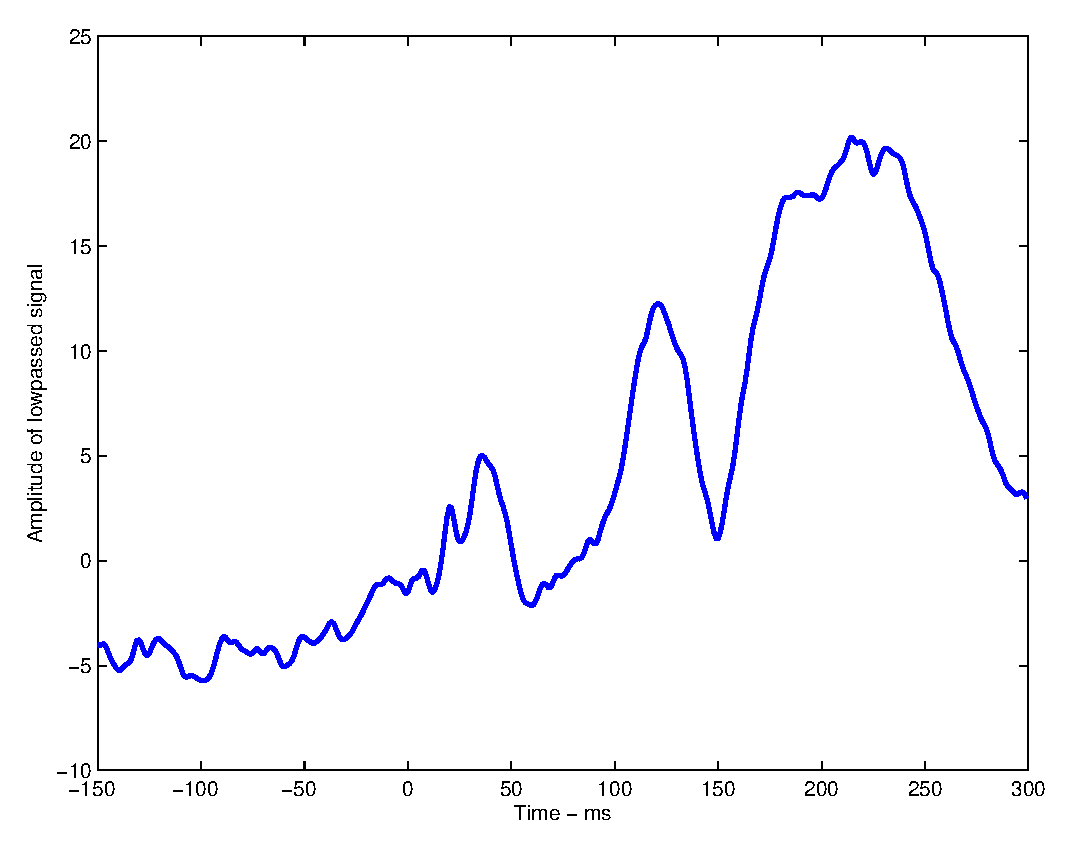
\includegraphics[width=11pc]{MeanLowpassedAmp.eps}
\caption{\label{label}Temporal profile of amplitude of lowpassed LFPs at $200$ Hz around the target appearance which is indicated at $0$ ms.}
\end{minipage}\hspace{2pc}
\begin{minipage}{10pc}
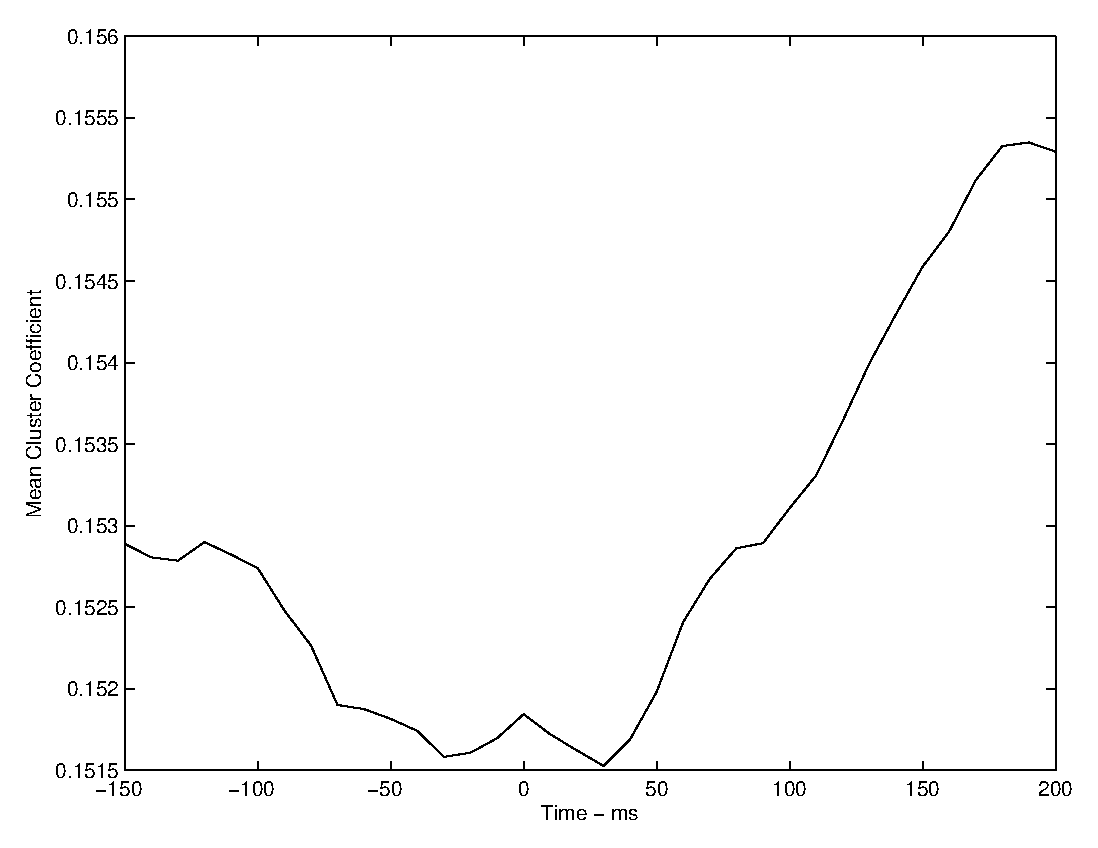
\includegraphics[width=11pc]{GrandMeanCC.eps}
\caption{\label{label}Temporal profile of cluster coefficients, $C$ for $\beta$ oscillation around the target appearance which is indicated at $0$ ms.}
\end{minipage} \hspace{2pc}
\begin{minipage}{10pc}
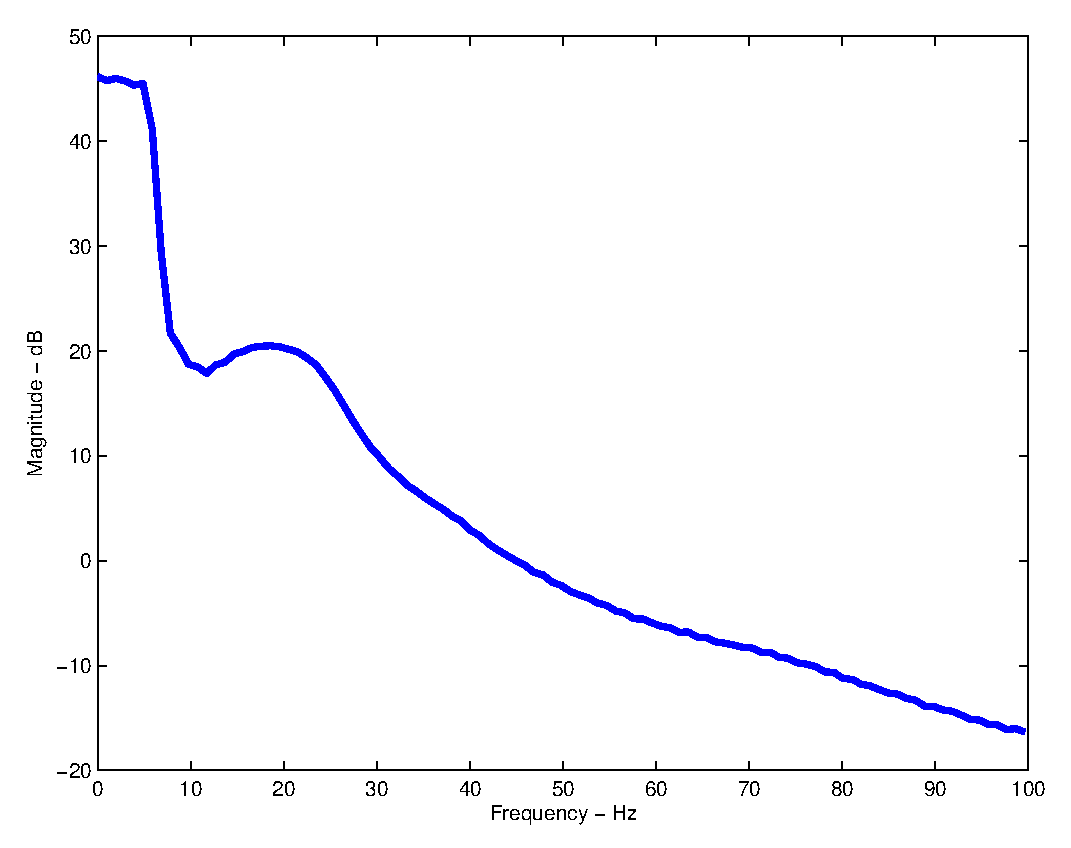
\includegraphics[width=11pc]{MeanPSD.eps}
\caption{\label{label}Averaged power spectrum of LFPs computed over $[-150,300]$ms around the target appearance for all used events.}
\end{minipage}

\begin{minipage}{10pc}
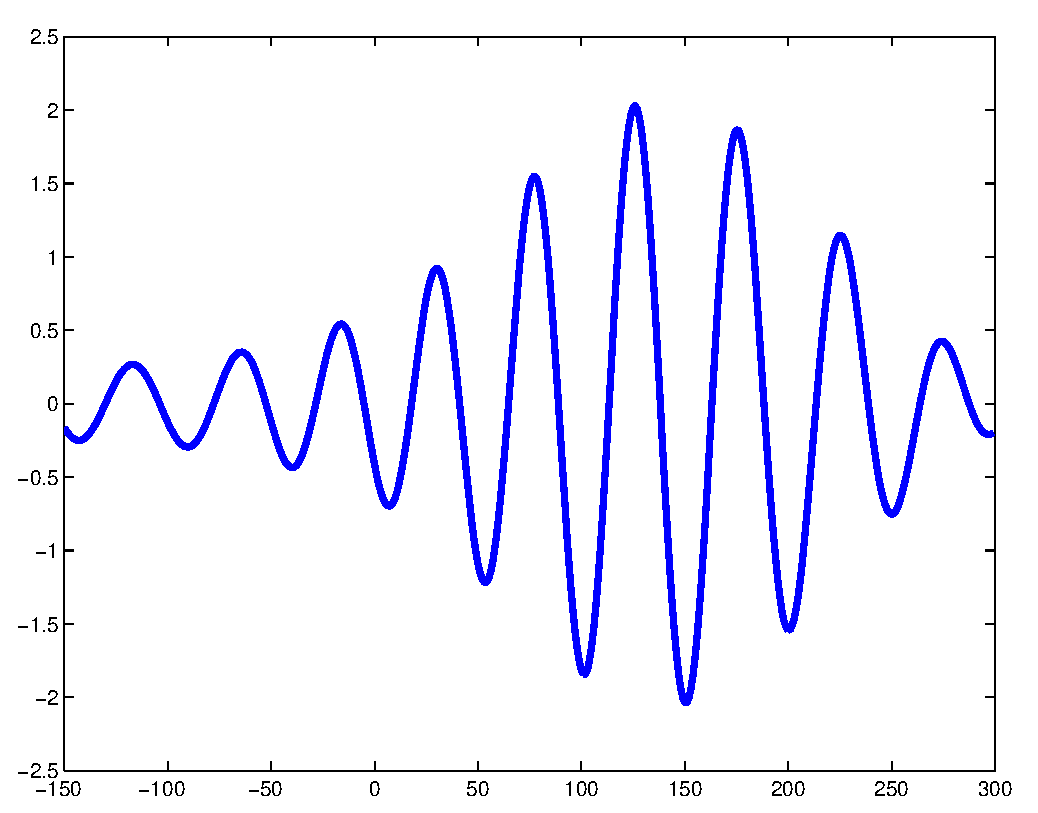
\includegraphics[width=11pc]{betaAMP.eps}
\caption{\label{label}Temporal profile of amplitude of $\beta$ oscillation around the target appearance which is indicated at $0$ ms.}
\end{minipage}\hspace{2pc}
\begin{minipage}{10pc}
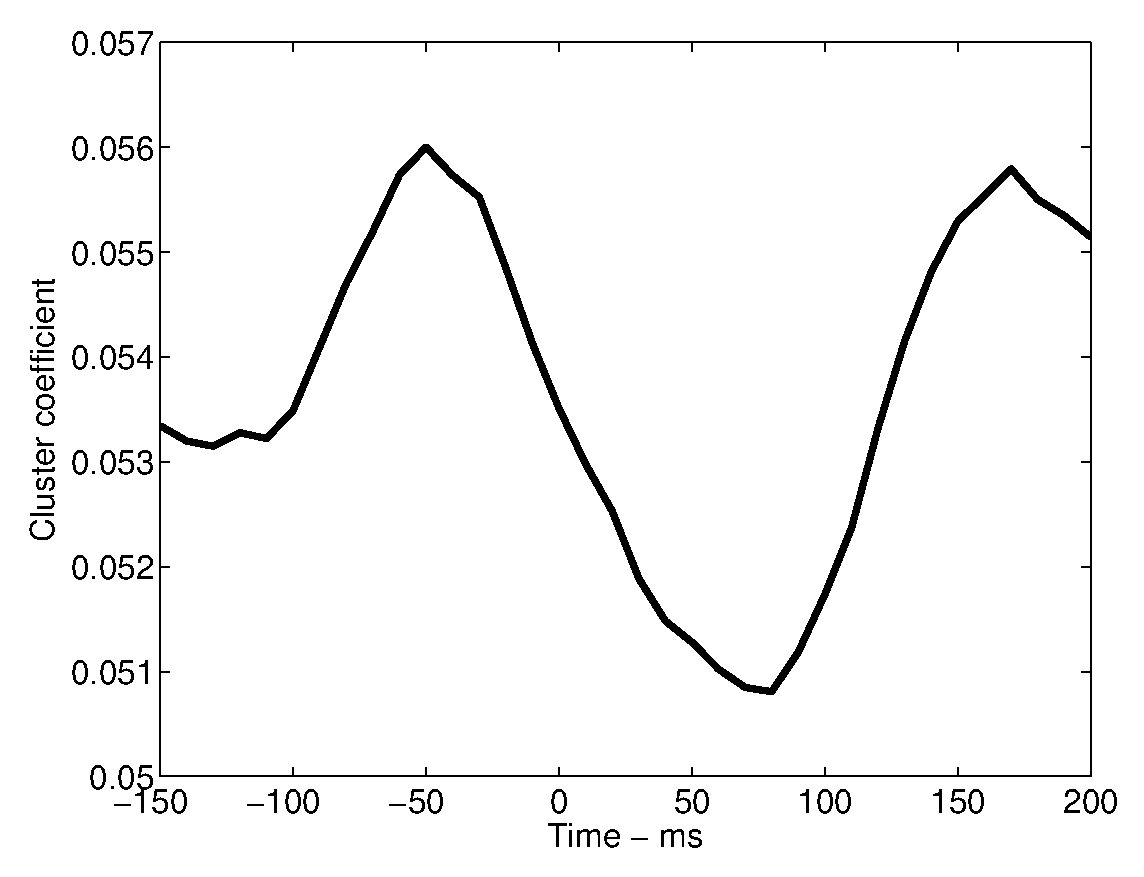
\includegraphics[width=11pc]{betaCCMean.eps}
\caption{\label{label}Temporal profile of cluster coefficients, $C$ for $\beta$ oscillation around the target appearance which is indicated at $0$ ms.}
\end{minipage}\hspace{2pc}
\begin{minipage}{10pc}
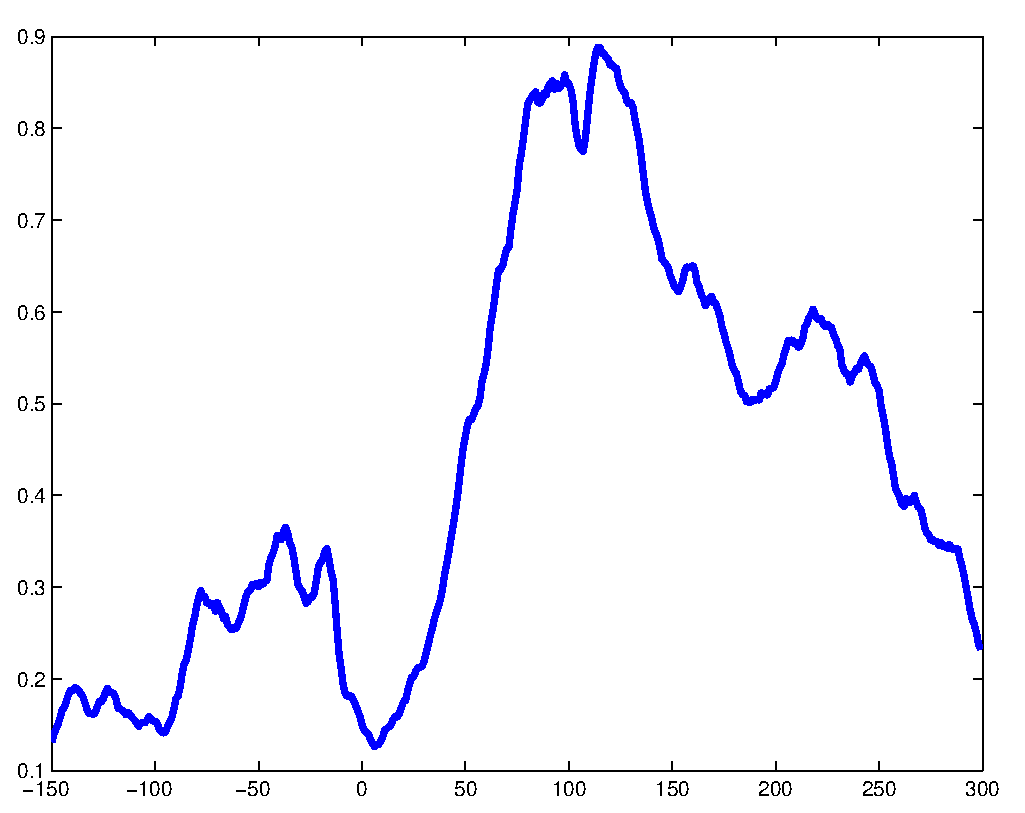
\includegraphics[width=11pc]{betaPPL.eps}
\caption{\label{label}Temporal profile of percentage of phase locking of $\beta$ oscillation around the target appearance which is indicated at $0$ ms.}
\end{minipage} 
\end{figure}


\subsection{Spatiotemporal profiles of cluster coefficients}

As shown in Fig.~\ref{fig:cnetwork}, most causal interactions were
detected for Time Window 2 than other two intervals. These
causality networks were obtained from the data set1, and we
obtained similar results using data sets 2 and 3 as well. In order
to look into the causality network consistency over data sets, we
plotted the degrees of all neurons for 3 data sets in
Fig.~\ref{fig:degree}.  All data sets had similar distributions of
degrees and same `hub' neurons 9 and 15 - neurons with unusually
high degree. Interestingly neurons recorded from a same electrode
were not interacting with one another, but they were causally
influencing on neurons from different electrodes.

\begin{figure}[ht!]
\begin{center}
\includegraphics[width=6.5in]{LPSpatiotemporal.eps}
\end{center}
\caption{Cluster coefficients of lowpassed signals of each channels over time around the target appearance mapped to their anatomical locations over the array. R:Rostral, C:Caudal, M:Medial, and L:Lateral.}
\label{fig:STmapLP}
\end{figure}
\begin{figure}[ht!]
\begin{center}
\includegraphics[width=6.5in]{BetaSpatiotemporal.eps}
\end{center}
\caption{Same as Fig. \ref{fig:STmapLP}, but for $\beta$ range of LFPs.}
\label{fig:degree}
\end{figure}

\section{Discussions}
\label{sec:discussions}


\section{Acknowledgement}
The authors would like to thank M. Togawa, Y. Yamanishi, and N. Takahashi at NIPS and T. Umeda currently at department of neuroanatomy, Yokohama City University for surgery and training of monkeys. 

\bibliographystyle{IEEEbib}
\bibliography{refs}
\end{document}